\section{Example}
\label{sec:example}

To illustrate the educational potential of \oops\/, we present a worked-out example that models an exercise we have assigned to students of multi-agent systems in the past, at the Department of Artificial Intelligence at the University of Groningen.
We show how \oops' scripting can facilitate model construction and how its ability to visualize Kripke models can facilitate understanding of $S5_n$.
Our example concerns a simplified version of the `Wise Persons' puzzle:

\begin{quote}
There are two wise persons, Abelard (1) and Heloise (2). It is known to everyone that there are three hats: two red ones and one white one. The king puts a hat on the head of each of the two wise persons, who cannot see their own hat but can see the other person's hat (and they both know this). The king asks them sequentially if they know the color of the hat on their own head. The first person, Abelard, says that he does not know; the second person, Heloise, says that she knows.
Exercise: find out what must be the color of Heloise's hat.
\end{quote}

To model this problem,
let us define the propositions {\it r1} for `Abelard wears a red hat', {\it w1} for `Abelard wears the white hat', {\it r2} for `Heloise wears a red hat' and {\it w2} for `Heloise wears the white hat'.
In the full implementation of this example, available online,\footnote{\url{http://cloud.github.com/downloads/gertvv/oops/hats.lua}} a number of utility functions are given.
{\tt conj(f1, f2)} safely gives the conjunction of two formulas, {\tt knows(a1, f)} gives the formula $\square_{a1} f$' and {\tt knows2(a1, a2, f)} for $\square_{a1} \square_{a2} f$.
Finally, {\tt printAbelard(th)} and {\tt printHeloise(th)} give informative output on the knowledge states of Abelard and Heloise, given the theory {\tt th}.

The initial situation can be modelled by simply defining the basic facts given in the puzzle and stating that both Abelard and Heloise are aware of these facts to sufficient depth.
Of course, the background information should be common knowledge, but this is not possible in pure $S5_n$.
So we give knowledge to depth 2, the minimum level required to solve this puzzle.
The Lua code is as follows:
\begin{lstlisting}
-- each person has only one hat
oneHat = "(r1 = ~w1) & (r2 = ~w2)"

-- there is only one white hat
oneWhite = "(w1 > r2) & (w2 > r1)"

-- Abelard can see Heloise's hat
abelardSees = "#_1 w2 | #_1 r2"

-- Heloise can see Abelard's hat
heloiseSees = "#_2 w1 | #_2 r1"

-- background knowledge:
background = conj(conj(oneHat, oneWhite),
    conj(abelardSees, heloiseSees))

-- add the background and the wise persons'
-- knowledge about it (to depth 2)
th = oops.Theory()
th:add(background)
th:add(knows("1", background))
th:add(knows("2", background))
th:add(knows2("2", "1", background))
th:add(knows2("1", "2", background))
\end{lstlisting}
We can evaluate the agents' knowledge in the initial situation using the following statements:
\begin{lstlisting}
-- make sure we can show the counter-model
oops.attachModelConstructor()

print("Initial Situation: ")
printAbelard(th)
printHeloise(th)
oops.showModel()
\end{lstlisting}
The counter-model to Heloise knowing the color of her hat is shown in Figure~\ref{fig:output1}. The console output is as follows:
\lstset{language=}
\begin{lstlisting}
Initial Situation:
Abelard doesn't know
Heloise doesn't know
\end{lstlisting}
\lstset{language=lua}

\begin{figure}
\centering
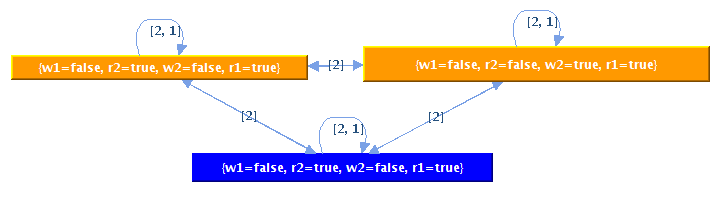
\includegraphics[width=0.4\textwidth]{images/demo04}
\caption{Counter-model to Heloise knowing the color of her own hat in the initial situation of the `wise persons' puzzle. The counter-model to Abelard knowing the color of his hat is almost identical, except that the relations between the worlds are for agent 1 (Abelard), not agent 2 (Heloise).}
\label{fig:output1}
\end{figure}

In the puzzle, Abelard is asked if he knows the color of his hat and responds that he doesn't. Heloise can now derive the color of her hat. We model this announcement by giving Heloise the knowledge that Abelard doesn't know the color of his hat.
\begin{lstlisting}
-- After Abelard announces he doesn't know:
abelardKnows = "#_1 w1 | #_1 r1"
th:add(oops.Formula("#_2 ~ F"):substitute(
    {F = abelardKnows}, {}))

print("After Abelard's announcement: ")
printAbelard(th)
oops.showModel()
printHeloise(th)
print("Consistent: " .. tostring(th:consistent()))
\end{lstlisting}
The output is as follows:
\lstset{language=}
\begin{lstlisting}
After Abelard's announcement:
Abelard doesn't know
Heloise knows his/her hat is red
Consistent: true
\end{lstlisting}
\lstset{language=lua}
Clearly, Abelard still doesn't know the color of his own hat (his own announcement doesn't help him), but Heloise is now aware that her hat is red, which is the correct solution to the puzzle.
The counter-model generated by the above code is nearly the same as the one shown in Figure~\ref{fig:output1}, so it is not shown separately.

This example demonstrates the kind of assignment that can be designed with  \oops\/.
It gives students the experience of using a theorem prover, and lets them experiment with different assumptions, providing insight into the formal logic that underlies a familiar riddle.
This can all be done quickly and easily due to \oops's integrated scripting facility and GUI.
